\graphicspath{{./figures/background/}}

\chapter{Background}

\section*{Chapter Overview}
\begin{itemize}
    \item The general structure of the EU liberalized electricity markets: players and roles.
    \item Harvesting wind power: first principles, main process stages and variables underlying power conversion, the central challenge of intermittency, forecasting as an approach for handling intermittency, major forecasting approaches.
    \item Time series forecasting: task definition, relevance, tasks categories, typical model requirements, methods and metrics for assessing model generalization performance, key requirements besides accuracy, examples of data-driven forecasting approaches, selecting models from a same approach.
    \item Spatio-temporal forecasting: enhancing models by going beyond exclusively temporal correlations, examples of approaches, how metrics are changed.
\end{itemize}
\pagebreak

\section{Liberalized Electricity Markets}

In a liberalized electricity market, multiple entities are involved in supplying energy to final consumers, as \ref{fig:electricity_grid_players} illustrates.
In the EU, these parties are electricity generators, transmission system operators (TSO), distribution system operator (DSO), electricity supplier, and regulator \cite{erbach2016market}.
TSOs are responsible for long-distance transport of energy and for balancing supply and demand in timeframes under quarter-hour. Imbalances of this nature cause deviations from the nominal frequency and shortages in more severe cases.
DSOs are responsible for delivering electricity to consumers.
Electricity suppliers buy energy from generator parties and resell it to consumers.
The liberalized EU grid system counts yet with another kind of entity, the balance responsible parties (BRPs), which although not directly involved in neither production nor in consumption activities, are financially responsible for the supply-demand balance \cite{erbach2016market}.

\begin{figure}[H]% H manda colocar exatamente nessa posição no texto (relativa aos parágrafos anterior e posterior)
	\centering
    \caption{The different stages of electricity supply and the responsible parties in a liberalized market.}
    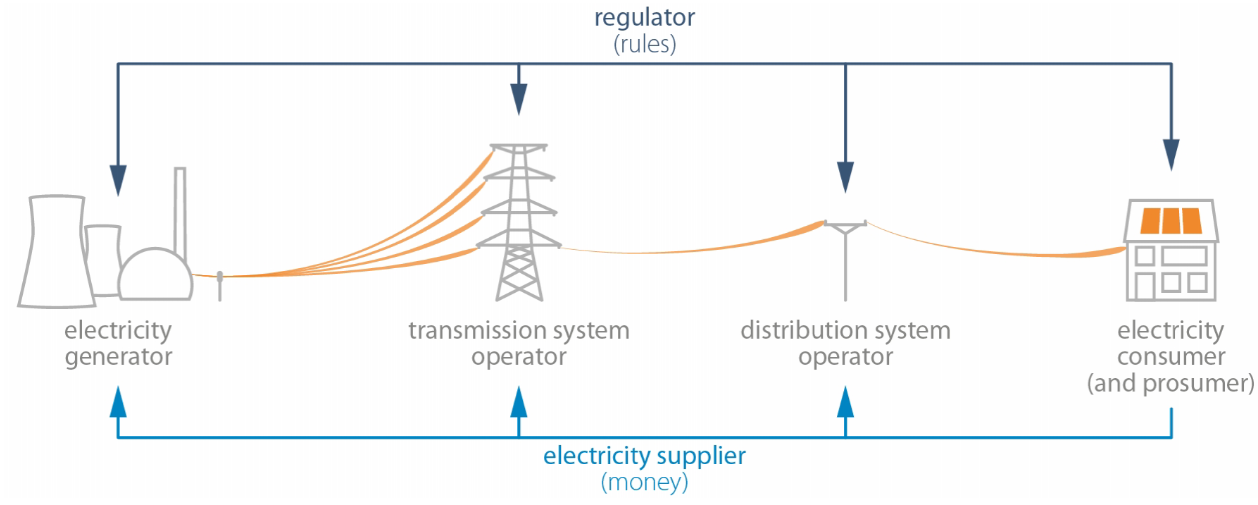
\includegraphics[scale=0.35]{electricity_grid_players.png} \\
    \raggedright
    Source: Adapted from \cite{erbach2016market}.
	\label{fig:electricity_grid_players}
\end{figure}

\section{Wind Power Generation}

In 1920, Betz \cite{betz1920limit} modeled a generic wind harvesting system as an open-disc actuator and, by using the energy conservation equation for a stream tube flowing through this disk, he derived an upper limit for the power harvested by a horizontal-axis wind turbine. The \textit{Betz Limit}, as it is known, is a function of rotor diameter $D$ (via the rotor swept area $A$) and the average free stream wind velocity $v$ at hub height $H$ (eq. \ref{eq:power-ideal}).
\begin{equation}\label{eq:power-ideal}
P_{ideal} = \frac{1}{2}\rho \cdot A(D)\cdot v^3
\end{equation}

Due to losses such as those associated to (1) momentum deficit in lower atmosphere boundary layer, (2) wakes from neighboring turbines, (3) suboptimal yaw angle and (4) blade tip vortices, the power harvested by the turbine rotor is only a fraction $C_p$ (coefficient of power) of this idealized maximum. Further  losses (a) of mechanical nature in the interfaces rotor-gearbox and gearbox-generator (\ref{fig:wind_power_conversion_stages}), (b) of electrical nature in the interface generator-converter  are modeled by the fractions $\eta_{m}$ and $\eta_{e}$, respectively,  to yield the actual power generation as measured at the power converter, \ref{eq:power_real} \cite{albadi2009capacity}.
\begin{equation}\label{eq:power_real}
P = C_p\eta_{m} \eta_{e}  \cdot \frac{1}{2}\rho \cdot A(D)\cdot v^3
\end{equation}

In this equation, $D$ and $H$ are design variables. The air density $\rho$ may vary during operation due to changes in air temperature, but its effects are often negligible. Finally, $C_p$, $v$ depend both on design (e.g., hub height $H$, blade profiles) and operation conditions (e.g., velocity speed and direction).
\begin{figure}[H] % H manda colocar exatamente nessa posição no texto (relativa aos parágrafos anterior e posterior)
	\centering
    \caption{ The different stages of the overall wind power conversion process. }
    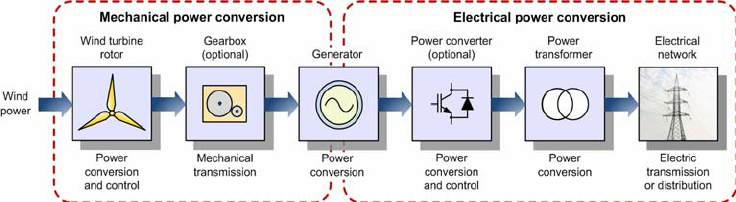
\includegraphics[scale=0.6]{wind_power_conversion_stages.png} \\
    \raggedright
    Source: Adapted from \cite{molina2011modelling}.
	\label{fig:wind_power_conversion_stages}
\end{figure}


In operation, the dominant source of variability for the generated power is $v$. Being climate and weather-dependent, it is also the main reason for the intermittency and non-dispatchability of wind power \cite{demeo2006natural}. This dependence motivates the usage by designers and generation operators of the so-called \textit{wind-to-power curves} (or \textit{power curves}), which are semi-empirical relations that allow one to determine the generated power $P$ by knowing the wind velocity $v$.

As design, planning, operation, maintenance, and trading of wind power are subject to such high variabilities, forecasting wind power generation (WPG) provides value for the different players in the electricity grid, illustrated in \ref{fig:electricity_grid_players}. Table \ref{tab:forecasting_interests} gives some examples of how various system operation aspects may profit from forecasts at different time scales.

\begin{table}[h]
    \centering
    \caption{Forecasting horizons in WPG and their main applications.}
    \begin{tabular}{ccc}
        \hline
        \begin{tabular}[c]{@{}c@{}}Forecasting\\ Horizon\end{tabular} & Definition             & Applications                                                         \\ \hline
        Very Short                                                    & $\sim secs\ - 0.5h $   & turbine control, load tracking          \\
        Short                                                         & $0.5h - 72h$           & pre-load sharing                                                     \\
        Medium                                                        & $72h\ – 1\ week $      & power system management, energy trading \\
        Long                                                          & $1\ week\  – 1\ year $ & turbines maintenance scheduling                                      \\ \hline
    \end{tabular}
    \label{tab:forecasting_interests}
\end{table}

Power generation from single turbines can also be aggregated at different levels.
Market operators, for example, profit the most from regional aggregations, since for energy trading, this resolution is sufficiently high, with higher resolutions across the same space scales of interests often too costly \cite{jung2014forecasting}.
In countries such as Germany, where continental and national renewables-promoting public funding initiatives such as the \textit{Energiewende} resulted in high penetration of wind power in the grid, forecasting wind power generation accurately has a tangible impact both environmentally and economically.


The intermittency of renewables motivated an alternative measure of power generation: the \textit{capacity factor} (CF).
CF is defined as the ratio of the actual generated power and the installed capacity. When considering WPG data across long timespans for both analysis and forecasting, it is usual that new commissionings take place, which manifests itself as a step perturbation into the overall generated power. In this case, CF can be useful as it is mostly insensitive to single new commissionings.
Climate and weather-conditioned local wind velocities imply for the power generation not only significant temporal dependencies but also significant spatial dependencies. As air masses influence one another in different scales, wind power generation in neighboring turbines tends to present higher correlations than turbines distant from one another \cite{engeland2017variability}. Therefore, wind power generation is a phenomenon with dominant spatio-temporal dependencies.
Usual approaches to forecasting wind power generation are physical, statistical, and machine learning-based \cite{jung2014forecasting}. The physical approach relies on the modeling of the power curve using Computational Fluid Dynamic (CFD) models, taking Numerical Weather Prediction (NWP) as inputs for defining the boundary conditions. The main limitations of this approach are (a) the high costs involved in the development of such models, along with (b) the large uncertainties entailed by the NWP data. The statistical approach uses historical data and statistical time series models to produce forecasts for wind speed, which is then used in the power curve for forecasting the power generation itself. Finally, in machine learning approaches, one uses historical data for wind speed or power generation, eventually combined with historical data of weather conditions to forecast either (a) local wind speeds, with their subsequent transformation into generated power via power-curve or (b) generated power directly.

\section{Time Series Forecasting}

In \cite{brockwell1996introduction}, Brockwell \& Davis define time series as ``a set of observations $y_t$, each one being recorded at a specific time $t$.'' When observations are recorded at discrete times, they are called a discrete-time time series, on which we focus this work.

An important task in time series analysis is time series forecasting, which concerns ``the prediction of data at future times using observations collected in the past'' \cite{hyndman2018principles}. Time series forecasting permeates most aspects of modern business, such as business planning from production to distribution,  finance and marketing, inventory control, and customer management \cite{oreshkin2019nbeats}. In some business use cases, a single point in forecasting accuracy may represent millions of dollars \cite{kahn2003measure, jain2012answers}.

Time series forecasting tasks can be categorized in terms of (a) inputs, (b) modeling, and (c) outputs. In terms of inputs, one can use exogenous features or not, one or more input time series (univariate \textit{versus} multivariate). In terms of modeling, one must define a resolution (e.g., hourly, weekly), can aggregate data in different levels (hierarchical \textit{versus} non-hierarchical), and can use different schemes for generating models (we distinguish statistical from machine learning-based). Finally, regarding outputs, a forecasting task might involve making predictions in terms of single values or whole distributions (deterministic \textit{versus} probabilistic), point-predictions or prediction intervals, predict values for either a single point or for multiple points in future time (one-step-ahead \textit{versus} multi-step-ahead). In this work, we focus on deterministic, one-step ahead point forecasting, where one is interested in obtaining a function $f: \mathbb{R}^T \rightarrow \mathbb{R}$ (a \textit{forecasting model}) that maps historical observations  $\boldsymbol{y} _{1:T} = \{y_1,…,y_T\}$ of a variable $y_t$ to its value in a future time step $T+h$, for a forecasting horizon of interest $h$.

The main requirement for a forecasting model concerns the accuracy of its forecasts $\hat{y}_{t|T}$. This accuracy is quantified by a \textit{metric}, which summarizes the distribution of the forecast error $e_{t} = y_{t} - \hat{y}_{t|T}$ over the different evaluation timesteps $t$. In the following subsections, we introduce some typical options for (a) schemes for defining the evaluation timesteps $t$ (\ref{subsec:model_evaluation}), (b) accuracy metrics (\ref{subsec:metrics}), as well as (c) approaches for generating  forecasting models (\ref{subsubsec:baseline_methods}, \ref{subsubsec:statistical_methods}, \ref{subsubsec:ml_methods}).

\subsection{Model Evaluation}\label{subsec:model_evaluation}

Assessing the performance of a model $f$ requires defining the time indexes $t$ for evaluating the forecast errors $e_{t}$ . In a naive approach, one could use all available data for both model inference and evaluation. This would, however, result in a highly biased estimate of the model generalization performance. Less biased estimations could be attained instead by partitioning the available dataset into a \textit{training dataset} $\boldsymbol{y} _{1:T} = \{y_1,…,y_T\}$, exclusive for model inference, and a \textit{test dataset} $\boldsymbol{y} _{T+1:T'} = \{y_{T+1},…,y_{T'}\}$, used for model evaluation (fig. \ref{fig:training_test_split}). Once an estimate for the model performance is attained, a separate model inference using both partitions can be carried out, so that the epistemic part of the generalization error, resulting from limited data in model inference, is kept at a minimum.
\begin{figure}[H]% H manda colocar exatamente nessa posição no texto (relativa aos parágrafos anterior e posterior)
	\centering
    \caption{Partitioning the available data in training and test datasets.}
    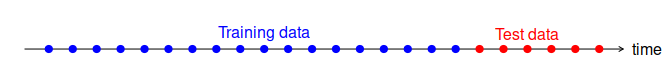
\includegraphics[scale=0.8]{traintest_split.png} \\
    \raggedright
    Source: Adapted from \cite{krispin2019handson}.
	\label{fig:training_test_split}
\end{figure}

Furthermore, it is necessary that this partitioning results in two sets of successive observations, in order to preserve the \textit{Markovian dependence} underlying the sequential observations. Even under this constraint, however, the choice on what point to split the data is still arbitrary, implying that assessing model performance on a single arbitrary choice would result in a biased estimate. To minimize this bias, the model performance can be assessed for several different splitting points. The partial results are then aggregated, typically by averaging, into an overall result of model performance. This procedure is known as \textit{out-of-sample cross-validation}.

As the forecast error generally increases for longer forecasting horizons, the out-of-sample estimate might overestimate the generalization error, especially if only one-step forecasts are of interest. For overcoming this, only the  first point in the test data is used in evaluating the error. This approach is known as \textit{expanding window cross-validation}, and is illustrated in \ref{fig:expanding_window_cv}.
\begin{figure}[H]% H manda colocar exatamente nessa posição no texto (relativa aos parágrafos anterior e posterior)
	\centering
    \caption{The expanding window cross-validation scheme.}
    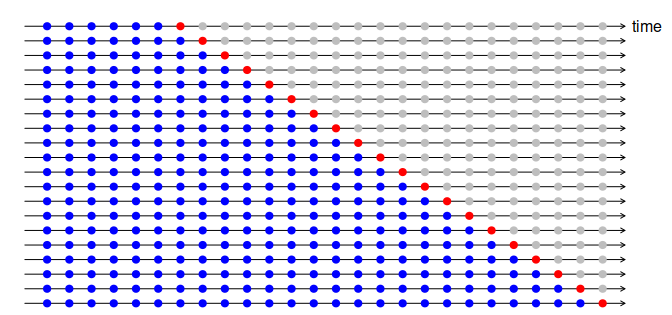
\includegraphics[scale=0.8]{expanding_window_cv.png} \\
    \raggedright
    Source: Adapted from \cite{krispin2019handson}.
	\label{fig:expanding_window_cv}
\end{figure}


\subsection{Accuracy Metrics}\label{subsec:metrics}
Many different metrics exist, each one summarizing the error distribution in a different way. Some of the most usual definitions  are presented from \ref{eq:rmse} to \ref{eq:mdrae} (see e.g., \cite{wu2019graphwavenet, liu2019st-mgcn, hyndman2006metrics}. In particular, $MASE$ and $MdRAE$ use as denominator the forecast errors of the naïve model, which takes the last known value to forecast the next point. The naïve model can be shown to be optimal for a random walk process \cite{hyndman2006metrics}.
\begin{equation}\label{eq:rmse}
    RMSE = \sqrt{\mathbb{E}(e_t^2)} = \sqrt{\frac{1}{(T'-T-1)}\sum_{t=T+1}^{T'} e^2_t}
\end{equation}

\begin{equation}\label{eq:mae}
    MAE = \mathbb{E}(|e_t|) = \frac{1}{(T'-T-1)}\sum_{t=T+1}^{T'} |e_t|
\end{equation}

\begin{equation}\label{eq:mape}
    MAPE = \mathbb{E}(|e_t/y_t|\cdot 100\%) = \frac{100\%}{(T'-T-1)}\sum_{t=T+1}^{T'} \left|\frac{e_t}{y_t}\right|
\end{equation}

\begin{equation}\label{eq:smape}
    sMAPE = \frac{100\%}{T'-T-1}\sum^{T'}_{T=T+1} \frac{|e_t|}{(|y_{t}|+|\hat{y}_{t}|)/2}
\end{equation}

\begin{equation}\label{eq:mdape}
    MdAPE = q_{0.5}(|e_t/y_t|\cdot 100\%)
\end{equation}

\begin{equation}\label{eq:smdape}
    sMdAPE = q_{0.5}\left(200\% \cdot \frac{|e_t|}{y_{t}+\hat{y}_{t}}\right)
\end{equation}

\begin{equation}\label{eq:mase}
    MASE = \mathbb{E}\left(\left|\frac{e_t}{e_{t, na\ddot{i}ve}}\right|\right)
\end{equation}

\begin{equation}\label{eq:mdrae}
    MdRAE = q_{0.5}\left(\left|\frac{e_t}{e_{t, na\ddot{i}ve}} \right|\right)
\end{equation}


By summarizing the forecast error distribution into a reduced set of values, forecasting metrics are essential in model development as well as in method development.  To forecasters (model developers) and forecast users, metrics offer  a concise, unambiguous way to communicate accuracy requirements and specifications. For methods developers, it allows comparing different methods across different use cases, forecasting settings, and datasets.

On the one hand, single metrics concisely convey information about the error distribution, which is useful for comparing models and making decisions. On the other hand, a single metric cannot convey all aspects of the error distribution, and often using more than one metric becomes necessary to ensure sufficiency \cite{armstrong2002principles}. Therefore, deciding on a group of metrics often involves a trade-off between conciseness and sufficiency.

Metrics differ in interpretability, scale invariance, sensitivity to outliers, symmetric penalization of negative and positive errors, and smoothness as $y_t$ approaches zero \cite{hyndman2006metrics}. Therefore, it is important that the choice on the metrics set is coherent with the application requirements \cite{armstrong2002principles}. For example, while failing to forecast single sudden peaks in local wind speed (wind gusts) might not be important in wind farm planning, it might be a primary requirement for wind turbine operation.
Table \ref{table_metrics} summarizes sensitivities for the presented metrics.
\begin{table}[h]
    \centering
    \caption{Forecasting accuracy metrics and their sensitivities to scale and outliers.}
    \label{table_metrics}
    \resizebox{\textwidth}{!}{%
    \begin{tabular}{llcccc}
        \hline
        Alias  & Name                                       & \begin{tabular}[c]{@{}c@{}}Scale\\ Sensitivity\end{tabular} & \begin{tabular}[c]{@{}c@{}}Outliers\\ Sensitivity \end{tabular} & \begin{tabular}[c]{@{}c@{}}Smoothness\\at $y_t \rightarrow 0$ \end{tabular} & \begin{tabular}[c]{@{}c@{}}Symmetry\\at $e_t=0$ \end{tabular} \\ \hline
        RMSE   & Root Mean Squared Error                    & \fullcirc                                    & \fullcirc                                       & \fullcirc                  & \emptycirc \\
        MAE    & Mean Absolute Error                        & \fullcirc                                    & \fullcirc                                       & \fullcirc                  & \emptycirc \\
        MASE   & Mean Absolute Scaled Error                 & \emptycirc                                   & \fullcirc                                       & \fullcirc                  & \emptycirc \\
        MAPE   & Mean Absolute Percentual Error             & \emptycirc                                   & \fullcirc                                       & \emptycirc                 & \emptycirc \\
        MdAPE  & Median Absolute Percentual Error           & \emptycirc                                   & \emptycirc                                      & \emptycirc                 & \emptycirc \\
        sMAPE  & Symmetric Mean Absolute Percentual Error   & \emptycirc                                   & \emptycirc                                      & \emptycirc                 & \fullcirc \\
        sMdAPE & Symmetric Median Absolute Percentual Error & \emptycirc                                   & \emptycirc                                      & \emptycirc                 & \fullcirc \\
        MdRAE  & Median Relative Absolute Error             & \emptycirc                                   & \emptycirc                                      & \fullcirc                  & \emptycirc \\ \hline
    \end{tabular}
    }
\end{table}

Although often the most important one, accuracy is often just one of many requirements in a forecasting model development. In \cite{armstrong2002principles}, Armstrong reports that value inference time, cost savings resulting from improved decisions, interpretability, usability, ease of implementation, and development costs (human and computational resources) tend to be of comparable importance to researchers, practitioners, and decision-makers.

\subsection{Forecasting Approaches}

In general, forecasting approaches, statistical or machine learning-based alike, attain models by minimizing the forecast errors on the training set. This optimization process, often iterative, uses an optimization algorithm to update the model parameters configuration towards one that either (a) maximizes their likelihood or (b) minimizes a loss function on the training set.

The likelihood is, in essence, the relative number of ways that a configuration of model parameters can reproduce the provided data \cite{mcelreath2020rethinking}. In contrast, loss functions summarize the distribution of forecast errors, much like accuracy metrics. Loss functions are subject to an additional requirement, however, which is their suitability  as objective function in the convex optimization underlying most of model inferencing schemes. Therefore, although it is important that the objective function guiding the model inference is coherent with the metrics used for evaluating the models, they do not have to coincide. The Mean Squared Error (MSE, \ref{eq:mse}) is a typical choice for a loss function for continuous-type responses, as it accounts for both bias and variance errors, besides exhibiting smoothness amenable to convex optimization \cite{goodfellow2016deep}.
\begin{equation}\label{eq:mse}
    MSE = \frac{1}{T}\sum_{t=1}^T e^2_t
\end{equation}

Table \ref{tab:methods_overview} provides an overview of the approaches reviewed in this work. We start by presenting simple forecasting approaches\footnote[1]{Analogous to Murphy in \cite{murphy2012probabilistic}, we draw distinctions between the concepts of method, model, and model inference algorithm. A method can specify (1) how training data is used to generate a model (training, model inference, i.e., inference of its parameters) and (2) how a generated model uses its parameters and its input to make a prediction (inference). We denote by a model any unique configuration of parameters in a space defined by a method. Equivalently, a model represents a response surface (deterministic model) or the distribution of the response conditional on its inputs (probabilistic model).}, which are often used as baselines for other approaches \cite{hyndman2018principles}.

% Please add the following required packages to your document preamble:


\begin{table}[H]
    \caption{Forecasting approaches presented in this work. Most of these methods only model dependencies of temporal nature and are presented in this section. Exception are DCRNN, ST-GCN, and Graph WaveNet (ML-based), presented in section \ref{sec:stf}. They explicitly approach a more general forecasting setting where capturing both temporal and spatial dependencies is a central concern.}
    \centering
    \begin{tabular}{|ll|l|ll|}
        \hline
\multicolumn{2}{|c|}{\textbf{Statistical}}                                                                                                          & \multicolumn{1}{c|}{\textbf{Hybrid}} & \multicolumn{2}{c|}{\textbf{ML-based}}                                                                                               \\ \hline
\textbf{\begin{tabular}[c]{@{}l@{}}Exponential\\ Smoothing\end{tabular}} & \begin{tabular}[c]{@{}l@{}}SES\\ Holt's LinearHolt-Winter's\end{tabular} & \multirow{2}{*}{ES-RNN}              & \textbf{Temporal}                                                   & \begin{tabular}[c]{@{}l@{}}RNN\\ LSTM\\ N-BEATS\end{tabular}   \\ \cline{1-2} \cline{4-5}
\textbf{ARIMA}                                                           & \begin{tabular}[c]{@{}l@{}}AR\\ MA\\ ARIMA\end{tabular}                  &                                      & \textbf{\begin{tabular}[c]{@{}l@{}}Spatio-\\ Temporal\end{tabular}} & \begin{tabular}[c]{@{}l@{}}DCRNN\\ ST-GCN\\ GWNet\end{tabular} \\ \hline
\end{tabular}
    \label{tab:methods_overview}
\end{table}

\subsubsection{Baseline Approaches}\label{subsubsec:baseline_methods}

\noindent
\textbf{Naïve method} forecasts the signal as constant at its last observed value (eq. \ref{eq:naive}).
Here, the latest observation is the only important for forecasting \cite{hyndman2018principles}.
As the naïve forecast is the optimal prediction for a random walk process, it is also known as the \textit{random walk} method.
\begin{equation}\label{eq:naive}
    \hat{y}_{T+h|T} = y_T
\end{equation}

\noindent
\textbf{Seasonal Naïve method} models time series as harmonic with period $k$ observations (i.e., perfectly seasonal with seasonal period $k$), and for a given point  in future, suggest the corresponding last observed value from the last season (eq. \ref{eq:snaive}).
For example, all monthly forecasts for any future June assume the value from the last observed June value.
\begin{equation}\label{eq:snaive}
    \hat{y}_{T+h|T} = y_{T+h-k}
\end{equation}

\noindent
\textbf{Drift method.} The forecast for any point assumes a constant value rate of change, with values themselves starting from the latest observed value:
\begin{equation}\label{eq:drift}
    \hat{y}_{T+h|T} = y_{T} + h\left(\frac{y_T-y_1}{T-1} \right).
\end{equation}


\noindent
\textbf{Historical Average (HA) method.} The forecast for any point assumes a constant value: the average of the historical data (e.q. \ref{eq:ha}).
Here, all observations are considered to have equal importance in determining the forecast \cite{hyndman2018principles}.
\begin{equation}\label{eq:ha}
\hat{y}_{T+h|T} = \frac{1}{T}\sum_{t=1}^Ty_t
\end{equation}

\subsubsection{Statistical Approaches}\label{subsubsec:statistical_methods}

Statistical forecasting approaches are characterized by the modeling of the time series as a realization of a stationary stochastic process \cite{brockwell1990methods}, \cite{bontempi2013strategies}.
The two most widely used families of statistical methods are the Exponential Smoothing (ES) family and the ARIMA family \cite{hyndman2018principles}.

In the ES approach, the time series is modeled as combination of  interpretable components \cite{brockwell1990methods}.
In the \textit{classical decomposition} \cite{makridakis1997arma}, these components are trend component $m$, seasonal component $d$, and random noise (\textit{white noise}) $\varepsilon_t$, which are linearly combined to reconstruct the time series:
\begin{equation}\label{eq:ts_classical_decomp}
    y_t = m_t + s_t + a_t .
\end{equation}

We now describe some of the most known methods from the ES family.

\noindent
\textbf{SES (Simple Exponential Smoothing method)} forecasts by assigning importance at a maximum for the latest observed value, with exponentially decreasing importance to older observations (eq. \ref{eq:ses}).
In this sense, it is a compromise between the naïve method and the historical average method \cite{hyndman2018principles}.
Hyperparameter \footnote[1]{hyperparameters are parameters of the algorithms themselves, termed as such to distinguish them from (model) parameters. We discuss them in \ref{subsec:modelselection}}: $\alpha \in \mathbb{R}_{[0,1]}$.
\begin{equation}\label{eq:ses}
    \hat{y}_{t+1} = \alpha y_{t} + \alpha (1-\alpha) y_{t-1} + \alpha (1-\alpha)^2 y_{t-2} + ... = \alpha y_{t} + (1-\alpha) \hat{y}_{t}
\end{equation}

\noindent
\textbf{Holt's Linear method} features an additive trend component \cite{hyndman2008es}. Parameters: $(\alpha, \beta^*) \in \mathbb{R}^2_{[0,1]}$
\begin{equation}\label{eq:holt_linear}
    \begin{aligned}
    \hat{y}_{t+h|t} &= \ell_t + b_th, \\
    where\ \  \ell_t &= \alpha y_t + (1-\alpha)(\ell_{t-1}+b_{t-1}) \ \ \ \ \ \ (level) \\
    b_t &= \beta^*(\ell_t - \ell_{t-1}) + (1-\beta^*)b_{t-1} \ \ \ (growth)
    \end{aligned}
\end{equation}

\newpage
\noindent
\textbf{Holt-Winters' method} features additive trend and multiplicative seasonality components, for a seasonality length $m$, and forecasting horizon $h$.
Hyperparameter: $(\alpha, \beta^*,\gamma) \in \mathbb{R}^3_{[0,1]}$ (usual bounds, refer to \cite{hyndman2008es} for details).
\begin{equation}\label{eq:hs_method}
    \begin{aligned}
    \hat{y}_{t+h|t} = (&\ell_t + b_th)s_{t-m+h^+_m}, \\
    where \ \ell_t &= \alpha \frac{y_t}{s_{t-m}} + (1-\alpha)(\ell_{t-1}+b_{t-1})   &(level) \\
    b_t &= \beta^*(\ell_t - \ell_{t-1}) + (1-\beta^*)b_{t-1} &(growth) \\
    s_t &= \gamma y_t/(\ell_{t-1}+b_{t-1}) + (1-\gamma)s_{t-m} \ \ \ &(seasonal)
    \end{aligned}
\end{equation}

The other family of methods is the ARIMA (Autoregressive Integrated Moving Average) \cite{box1970distribution}.
Here, methods rely on repeatedly applying a difference operator to the observed values until the differenced series resemble a realization of some stationary stochastic process \cite{brockwell1990methods}.
We denote by $\nabla^k(\cdot)$ the difference operator of order $k$.
For $k=1$, $\nabla y_t = y_t - y_{t-1}$; for $k=2$, we have $\nabla^2(y_t) = \nabla(\nabla y_t) = \nabla y_t - \nabla y_{t-1} = y_t -2y_{t-1} + y_{t-2}$ and so forth.
Another useful notation in ARIMA methods is the \textit{backshift operator} $B^k(\cdot)$ with lag $k$.
For $k=1$, we have $B y_t = y_{t-1}$.
For $k=2$, $B^2(y_t) = B(B(y_t)) = y_{t-2}$.

\vspace{1em}
\noindent
\textbf{AR (Autoregressive) method.}  Linear regression with past values of the same variable (lagged values) as predictors.
A constant level $c$ and a white noise $\varepsilon_t \sim WN(\mu_\varepsilon, \sigma^2_\varepsilon)$ are considered.
Parameters: $\boldsymbol{\phi} = [\phi_1 \ \phi_2 \ \cdots \ \ \phi_p]^\top, \ \mu_\varepsilon, \ \sigma_\varepsilon, c$.
Hyperparameter: $p \in \mathbb{N}$.
\begin{equation}\label{eq:ar}
\hat{y}_t = c + \varepsilon_t + \phi_1 y_{t-1} + \phi_2 y_{t-2} + ... + \phi_p y_{t-p}
\end{equation}

\noindent
\textbf{MA (Moving Average) method.} Linear regression with lagged forecast errors $\varepsilon_\tau = \hat{y}_\tau - y_\tau$ as predictors.
Parameters:$\boldsymbol{\theta} = [\theta_1 \ \theta_2 \ \cdots \ \ \theta_q]^\top, \ \mu_\varepsilon, \ \sigma_\varepsilon, c$.
Hyperparameter: $q \in \mathbb{N}$.
\begin{equation}\label{eq:ma}
    \hat{y}_t = c + \varepsilon_{t} + \theta_1 \varepsilon_{t-1} + \theta_2 \varepsilon_{t-2} + ... + \theta_q \varepsilon_{t-q}
\end{equation}

\noindent
\textbf{(Non-seasonal) ARIMA method.} Linear regression, with lagged \textit{differenced} values $y_\tau'$ and lagged errors as predictors.
It combines autoregression on the differenced time series with a moving average model, hence the name \textit{Autoregressive Integrated Moving Average}, with \textit{integration} referring to the reverse operation of differencing, used when reconstructing the original time series from its differenced version.
Parameters: $\boldsymbol{\phi} = [\phi_1 \ \phi_2 \ \cdots \ \ \phi_p]^\top,\boldsymbol{\theta} = [\theta_1 \ \theta_2 \ \cdots \ \ \theta_q]^\top, \ \mu_\varepsilon, \ \sigma_\varepsilon, c$.
Hyperparameters: $(p, d, q)$. $p \in \mathbb{N^3}$
\begin{equation}\label{eq:arima}
\hat{y}'_t = c + \varepsilon_t + \phi_1 y'_{t-1} + ... + \phi_p y'_{t-p} + \cdots + \theta_1 \varepsilon_{t-1} + ... + \theta_q \varepsilon_{t-q}
\end{equation}

\pagebreak
\subsubsection{Machine Learning Approaches}\label{subsubsec:ml_methods}

Approaches solely based on Machine Learning struggled until recently to consistently outperform statistical time series forecasting approaches \cite{makridakis2018m4}.
Relying on biased evidence (e.g., models were evaluated across all time series without any criterious choice nor search for hyperparameters), Makridakis claimed in \cite{makridakis2018m4} that ``hybrid approaches and combinations of methods are the way forward for improving the forecasting accuracy and making forecasting more valuable.''
Oreshkin et al. challenged this conclusion in \cite{oreshkin2019nbeats}, introducing N-BEATS, a pure deep learning method that was shown to outperform statistical and hybrid methods, while also ensuring interpretability of intermediate outputs.

Below we present selected deep learning methods helpful for understanding current state-of-the-art approaches for both wind power generation-specific applications and in general univariate time series forecasting applications.

\vspace{1em}
\noindent
\textbf{RNN (Recurrent Neural Network)} uses the recurrent layer as building block: a cell that updates its state according to (a) its previous state $h_{t-1}$ and (b) its current input $x_t$ (fig. \ref{fig:rnn}). By performing this update at every timestep of a time series, this basic structure allows the RNN to express temporal dependencies in time series. An RNN can be built by serializing several of these self-looping cells between the input layer and the output layer for achieving higher-order mappings and thus capturing more complex temporal dependencies.
The major limitation of RNN in its basic design (recurrent layer as in \ref{fig:rnn}) is its inability to capture dependencies that span across longer periods than a few timesteps.
It arises from a phenomenon called \textit{vanishing gradients}: while inferring optimal parameters via gradient descent (learning phase), the gradients calculated via backpropagation through time become too small to guide the optimization \cite{paneru2015lstm}.
\begin{figure}[H]
	\centering
    \caption{The basic RNN architecture in its unfolded representation. Arrows indicate transfers of input and hidden states. Every block concatenates the last hidden state with the current input, passing the result to an activation function ($tanh$ in this illustration). The result is carried forward as the updated hidden state.}
    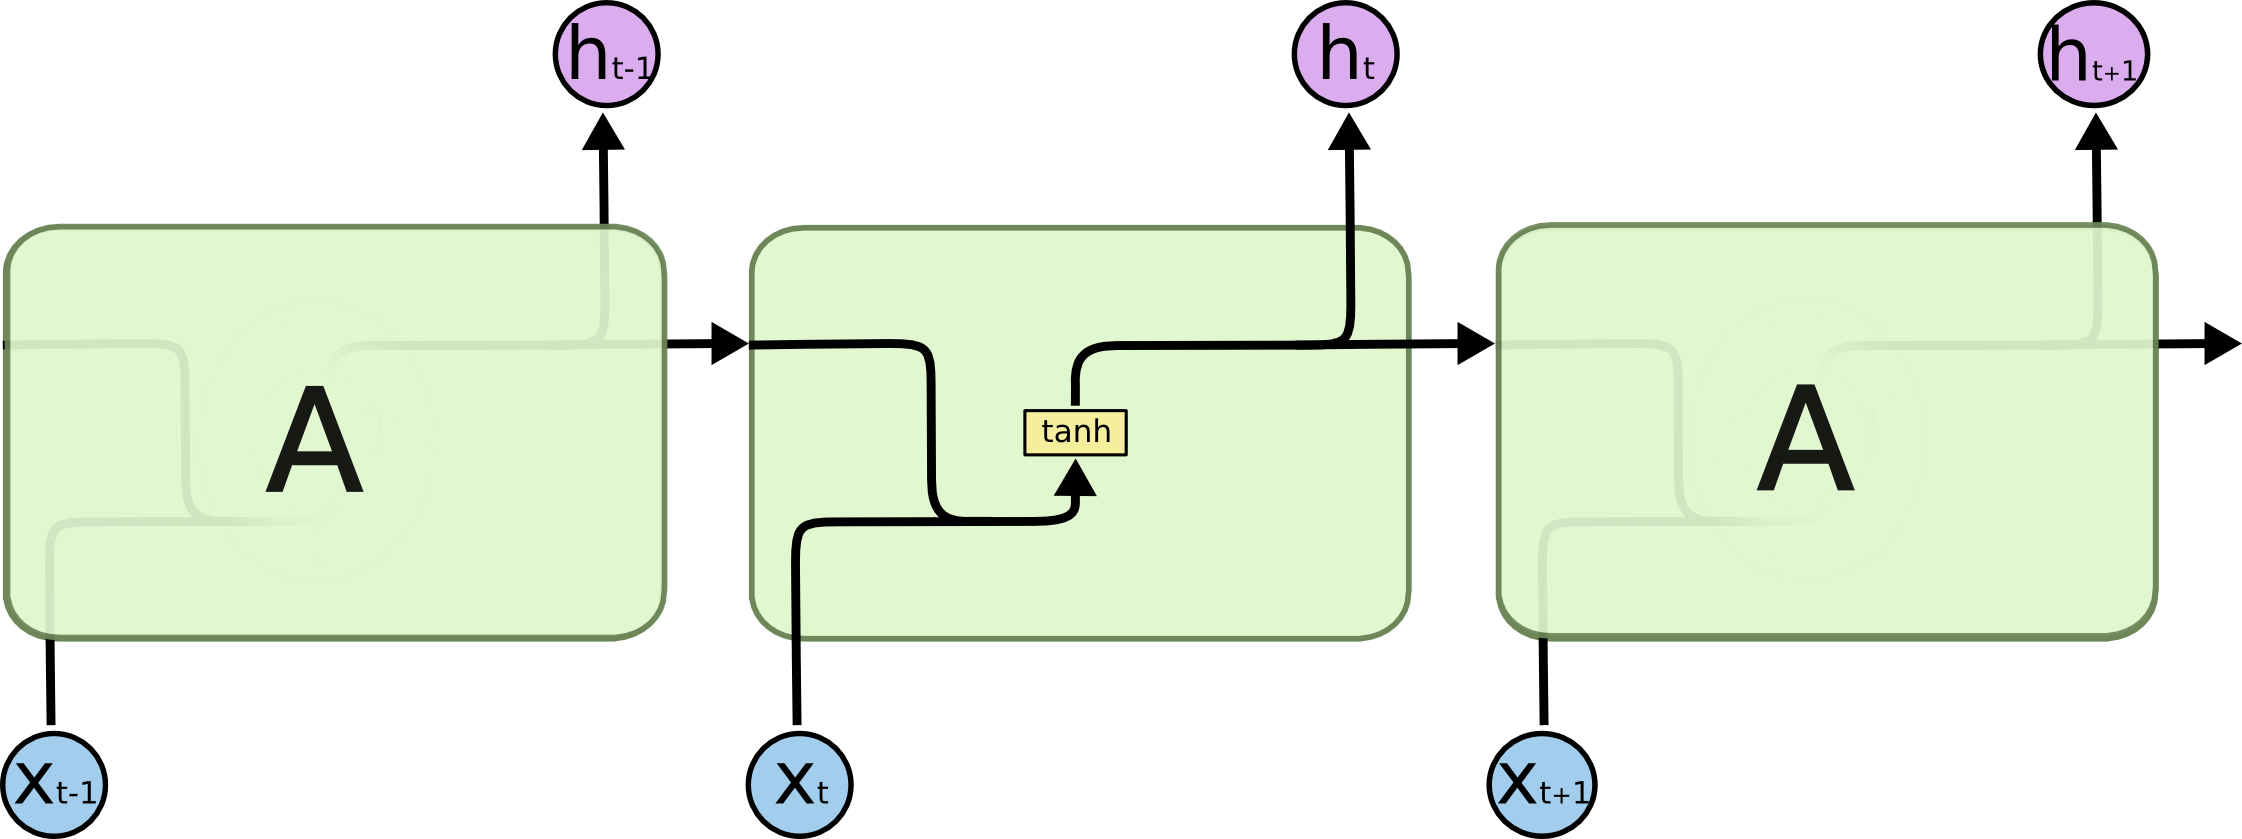
\includegraphics[scale=0.45]{rnn.png}  \\
    \raggedright
    Source: Adapted from \cite{paneru2015lstm}.
	\label{fig:rnn}
\end{figure}

\noindent
\textbf{LSTM (Long-Short Term Memory)} is a type of RNN, improving on its basic design most importantly by including an long memory state which is allowed to be transferred across several update steps with only minimal changes (superior horizontal line inside the repeating module in fig. \ref{fig:lstm}).
This allows information to persist across many cell updates, thus making it possible to capture long-term dependencies.
The extent to which this long memory state is preserved is controlled by forget gate, which we illustrate in figure \ref{fig:lstm} by the leftmost vertical path inside the cell.
The other paths represent other gated state transfers, which determine how (a) the previous cell state, (b) the previous long memory state and (c) the current cell inputs are combined and passed to the next cell iteration and as input to deeper layers \cite{paneru2015lstm}.
\begin{figure}[H]
	\centering
    \caption{Basic LSTM architecture in its unfolded representation. }
    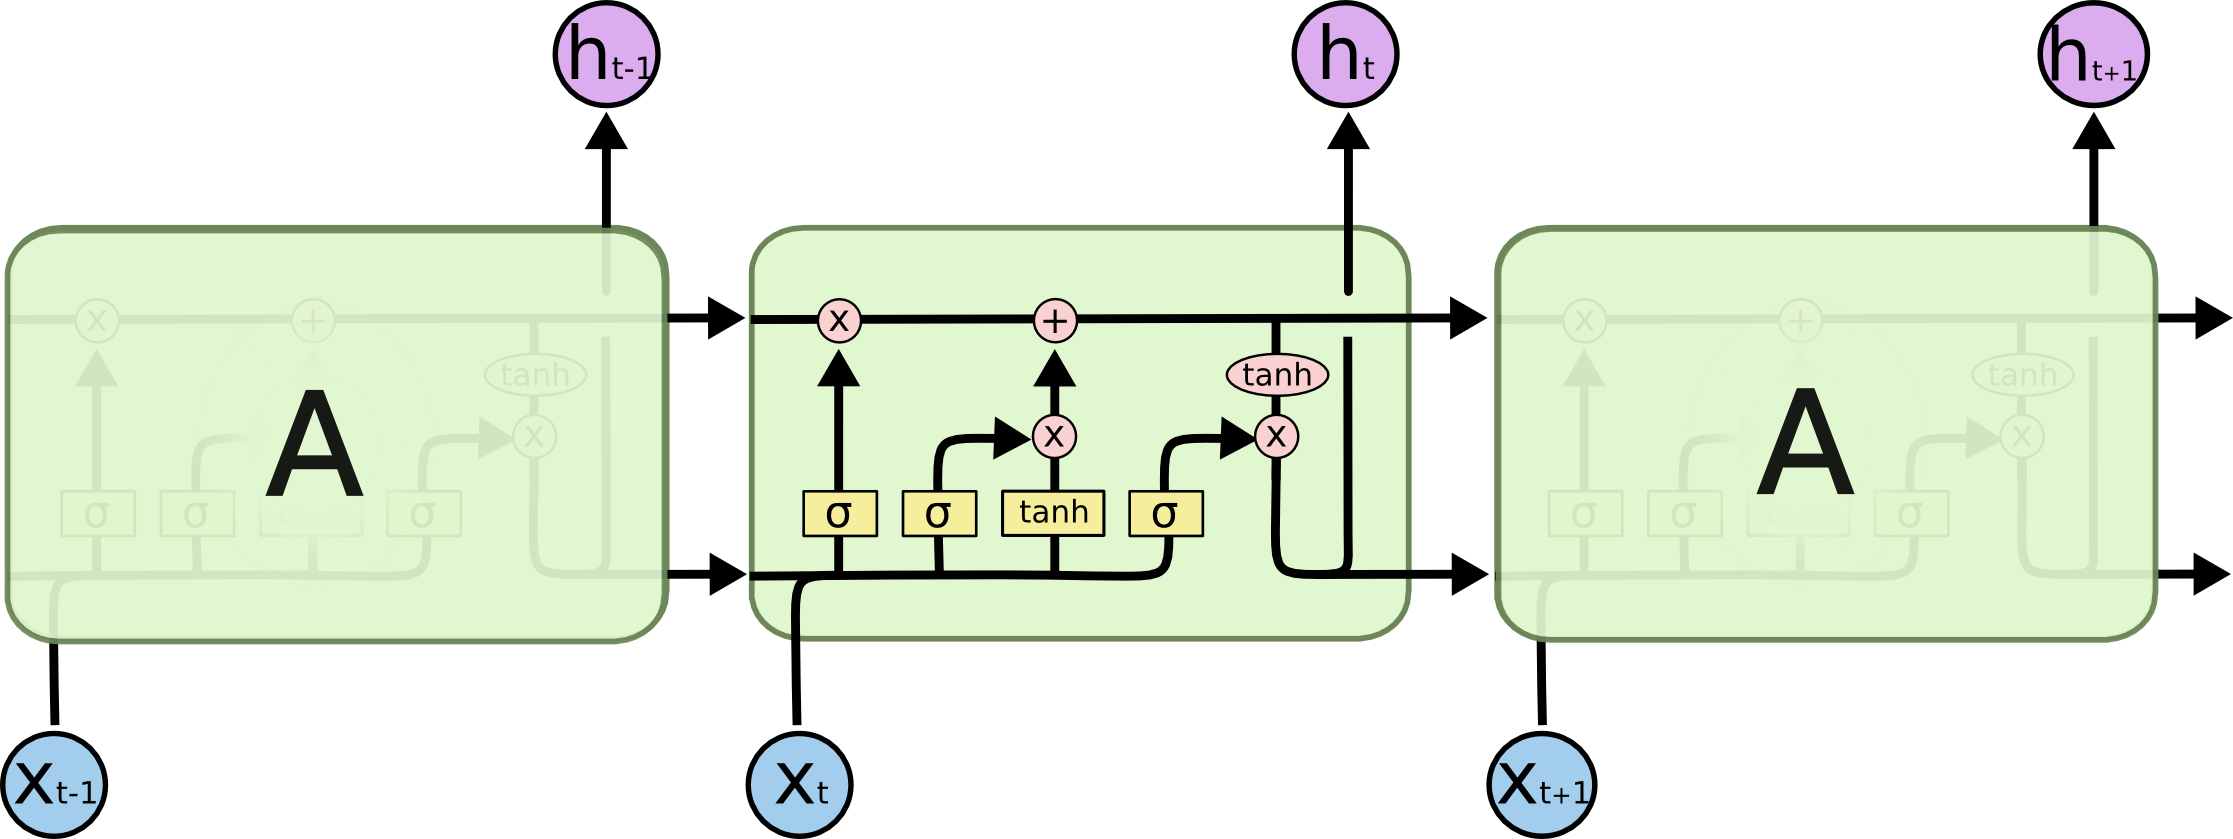
\includegraphics[scale=0.45]{lstm.png}  \\
    \raggedright
    Source: Adapted from \cite{paneru2015lstm}.
	\label{fig:lstm}
\end{figure}

\noindent
\textbf{NBEATS} uses as building block (a) a multi-layer fully connected network with ReLU nonlinearities, which feed (b) basis layers that generate a backcast and a forecast output.
Blocks are arranged into stacks, organized to form a model (fig. \ref{fig:nbeats}).
Models resulting from this architecture consistently outperformed state-of-the-art methods for univariate forecasting across different horizons and thousands of time series datasets of different nature, while using a single configuration of hyperparameters \cite{oreshkin2019nbeats}.
\begin{figure}[H]
	\centering
    \caption{NBEATS architecture.}
    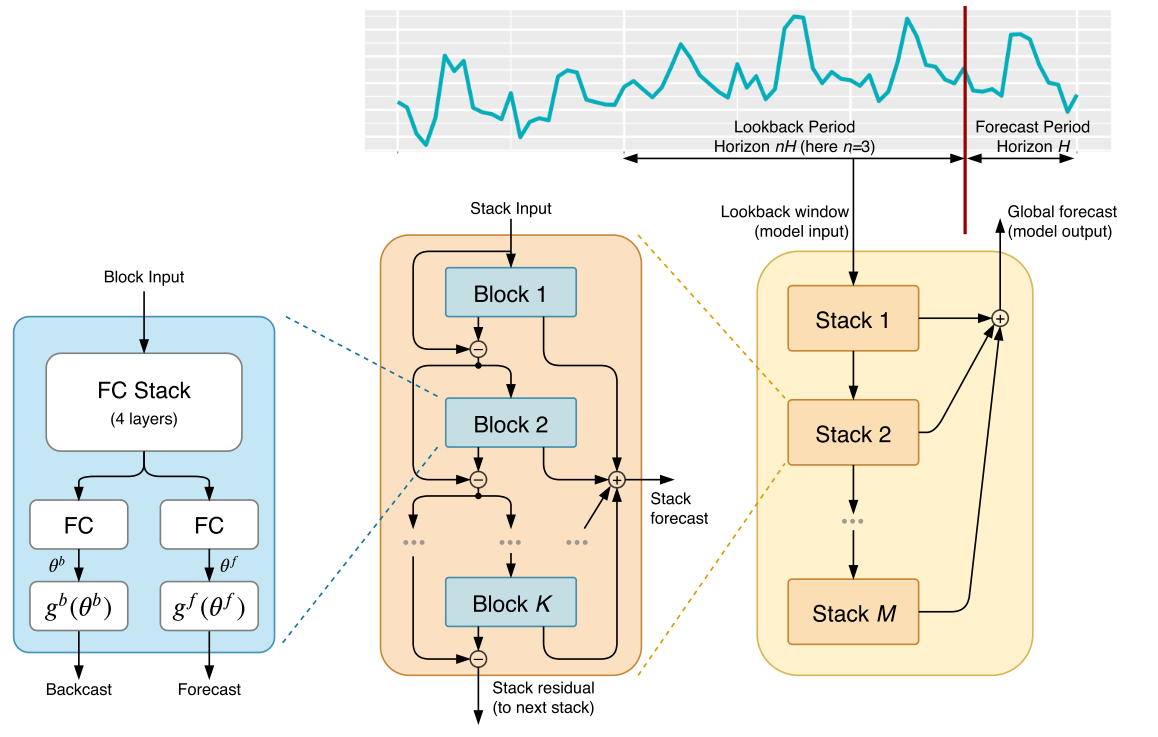
\includegraphics[scale=0.3]{nbeats.png}  \\
    \raggedright
    Source: Adapted from \cite{oreshkin2019nbeats}.
	\label{fig:nbeats}
\end{figure}

\subsubsection{Hybrid Approaches}
Hybrid methods combine machine learning and statistical approaches by using the outputs from statistical engines as features \cite{oreshkin2019nbeats}. Below we present ES-RNN, a hybrid method winner of the 2017 M4 forecasting competition.

\vspace{1em}
\noindent
\textbf{ES-RNN} uses Holt-Winters' ES method as statistical engine for capturing the seasonal and level components from the time series into features, which are then used as inputs by an LSTM model to exploit non-linear dependencies.
\begin{equation}\label{eq:esrnn}
    \begin{aligned}
    \hat{y}_{t+h|t} = LS&TM(y_t,\ell_t, s_t)\\
    where \ \ \ell_t &= \alpha \frac{y_t}{s_{t-m}} + (1-\alpha)\ell_{t-1}   &(level) \\
    s_t &= \gamma y_t/\ell_{t} + (1-\gamma)s_{t-m} \ \ \ &(seasonal)
    \end{aligned}
\end{equation}

\subsection{Model Selection}\label{subsec:modelselection}

As models have parameters, so do methods have their own, often referred to as \textit{hyperparameters}. They may control the space of model parameters configurations, the model inference process or eventually the loss function \cite{hutter2019automated}. Hyperparameters may have a major influence on the performance of resulting models. Accounting for this effect requires yet another partition in order to attain a minimally unbiased estimate of the resulting generalization error.
When working with three partitions, authors often denominate as:
\begin{itemize}
    \item (a) \textit{training set} the one used for model inference;
    \item (b) \textit{validation set}, the one for assessing model generalization error across multiple configurations of hyperparameters (i.e., for \textit{model selection});
    \item (c) \textit{test set}, the one for assessing the model generalization error for a \textit{specific} configuration of hyperparameters.
\end{itemize}

\pagebreak

\section{Spatio-Temporal Forecasting}\label{sec:stf}
In the spatio-temporal (ST) version of the forecasting task, one aims to attain a function $f: \mathbb{R}^{|V|\times T} \rightarrow \mathbb{R}^{|V|}$ that maps historical observations $\boldsymbol{y}_t = [y_{1,t}\  \  y_{2,t}\ \ \cdots \ \ y_{|V|,t}]^\top$ of a quantity across different regions to its value $\boldsymbol{y}_{t+1}$ in the next timestep  (eq. \ref{eq:stf}).
Often, regions are represented as vertices $v\in V$ in a graph $G$ modeling their spatial relationthips, in a process known as \textit{node embedding} \cite{liu2020intro}.

\begin{equation}\label{eq:stf}
    [\boldsymbol{y}_{t-T+1}, \  \cdots\ , \boldsymbol{y}_{t}] \xrightarrow{f(\cdot)} \boldsymbol{y}_{t+1}
\end{equation}

In some forecasting problems such as the weather-conditioned wind power generation, the spatial dependency might play an important along with the temporal dependencies themselves \cite{engeland2017variability}.
In this work, we distinguish between three different approaches to the ST forecasting problem.
In a naïve approach, time series for different locations are modeled independently, thus neglecting spatial dependencies.
In a second approach, the time series are modeled jointly via a multivariate forecasting approach, where for generating a single model one relies on historical observations not from a single but from several input variables, which can be expressed by a sequence of input vectors $\boldsymbol{X}_{1:T} = \{\boldsymbol{X}_1, ..., \boldsymbol{X}_T\}$.
Finally, we consider the explicit modeling of both spatial and temporal dependencies via dynamic graphs.
The latter approach is represented by the methods presented below.

\vspace{1em}
\noindent
\textbf{DCRNN (Diffusion Convolutional RNN).} improves RNN by replacing the matrix multiplication across recurrent layers by a diffusion convolution \cite{liu2020intro}.
Motivated by the traffic forecasting problem, where spatial dependencies are directional (non-Euclidean), Li et al. \cite{li2018dcrnn} recast the spatio-temporal evolution of a variable as a diffusion process on a directed graph, where every node corresponds to a sensor.
Learning is performed via (1) diffusion convolution, further integrated with a (2) seq-to-seq learning framework, and a (3) scheduled sampling for modeling long-term dependencies (fig. \ref{fig:dcrnn}).
\begin{figure}[H]
	\centering
 	\caption{The DCRNN architecture.}
	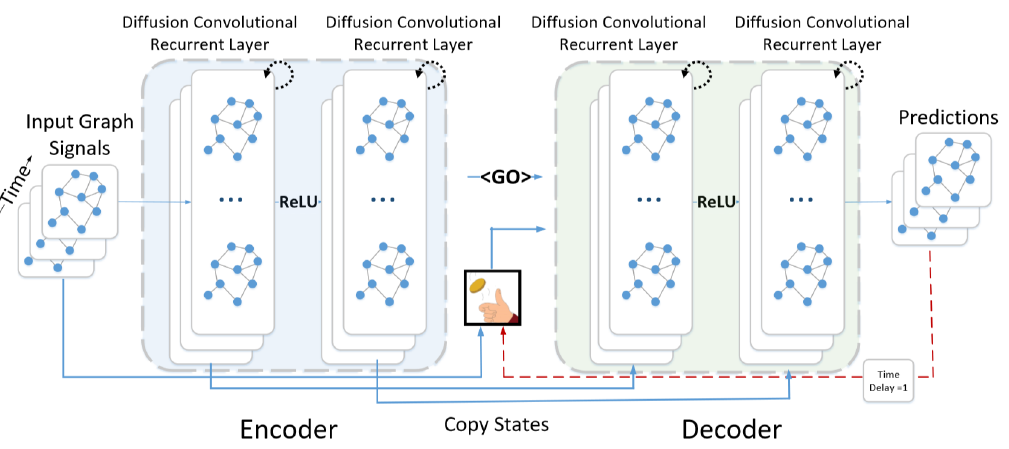
\includegraphics[scale=0.45]{dcrnn.png}  \\
    \raggedright
    Source: Adapted from \cite{li2018dcrnn}.
	\label{fig:dcrnn}
\end{figure}

\noindent
\textbf{ST-GCN.} A spatial-temporal graph is generated by stacking graph frames from all timesteps, each frame representing the graph state at a specific time (fig. \ref{fig:stgcn}).
The spatial-temporal graph is partitioned, and to each of its nodes is assigned a weight vector.
Finally, a graph convolution is performed on the weighted spatial-temporal graph.
\begin{figure}[H]
	\centering
 	\caption{ST-GCN underlying principle.}
	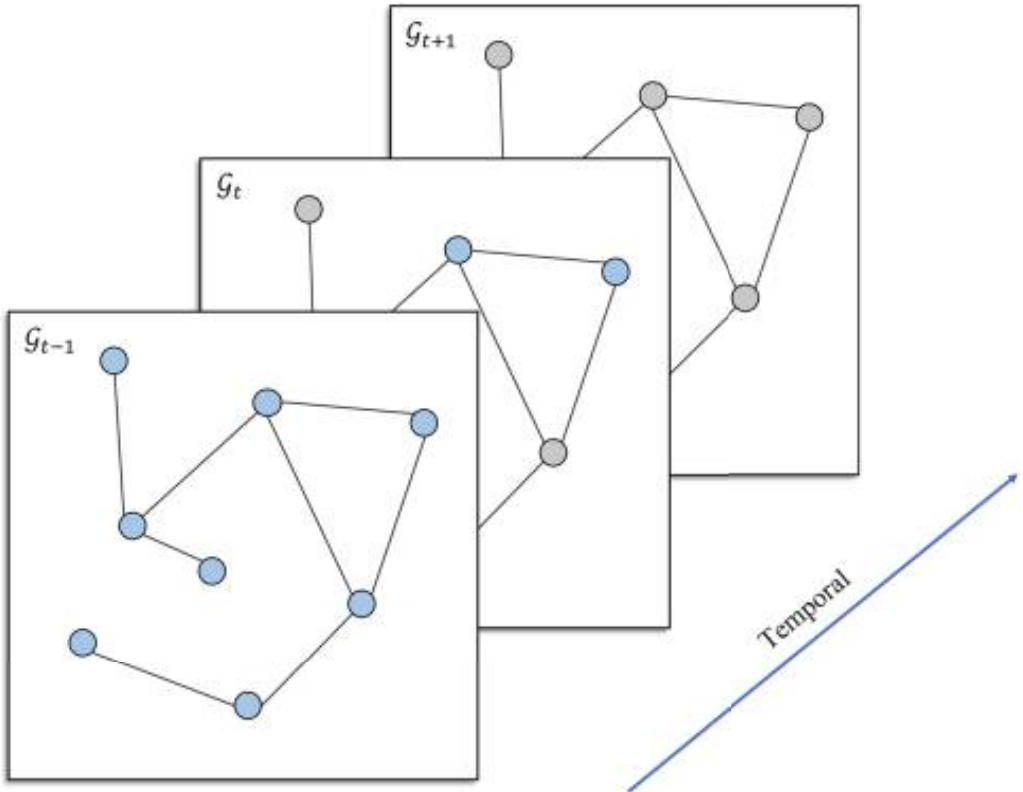
\includegraphics[scale=0.25]{stgcn.png}  \\
    \raggedright
    Source: Adapted from \cite{liu2019st-mgcn}.
	\label{fig:stgcn}
\end{figure}

\noindent
\textbf{GWNet.} The Graph Wavenet uses as building blocks a Temporal Convolution Network (TCN) and a Graph Convolution Network (GCN) for capturing temporal and spatial correlations respectively in every module.
As stacks of modules each capturing both spatial and temporal dependencies are used, this architecture allows models to capture correlations not exclusively temporal nor exclusively spatial.
Another core idea is the usage of a learnable self-adaptative adjacency matrix, which allows node dependencies to change over time and not necessarily be determined by their distances \cite{wu2019graphwavenet, liu2020intro}.
Euclidean distances $D_{ij}$ between every pair $(i,j)$ of districts are used just for initializing the adjacency matrix according to the Gaussian Kernel $A_{ij} = exp(-D_{ij}^2/2\sigma_{D}^2)$, which the authors normalize columnwise for faster convergence.
\begin{figure}[H]
	\centering
    \caption{The Graph Wavenet architecture.}
    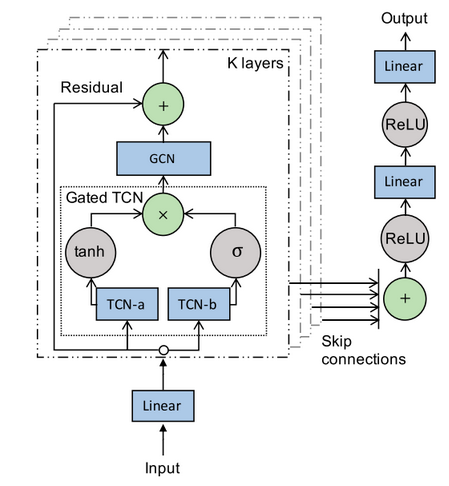
\includegraphics[scale=0.5]{graphwavenet.png}  \\
    \raggedright
    Source: Adapted from \cite{wu2019graphwavenet}.
	\label{fig:graphwavenet}
\end{figure}

\subsection{Accuracy Metrics}

The usual accuracy metrics in spatio-temporal forecasting are similar to their counterparts in the temporal setting, the main difference concerning the aggregation via averaging across space over the $v \in |V|$ regions, besides the aggregation across timesteps.
We present some of them in eqs. \ref{eq:mae}, \ref{eq:mape}, \ref{eq:rmse}.

\begin{equation}\label{eq:mae_multi}
    MAE = \frac{1}{|V|(T'-T-1)} \Sigma_{v=1}^{|V|} \Sigma_{t=T+1}^{T'} | \bm{\hat{y}}^{(v)}_{t} - \bm{y}_{t}^{(v)} |
\end{equation}


\begin{equation}\label{eq:mape_multi}
    MAPE = \frac{100\%}{|V|(T'-T-1)}\Sigma_{v=1}^{|V|} \Sigma_{t=T+1}^{T'} \frac{ | \bm{\hat{y}}^{(v)}_{t} - \bm{y}_{t}^{(v)} | }{ |\bm{y}_{t}^{(v)}| }
\end{equation}


\begin{equation}\label{eq:rmse_multi}
    RMSE = \sqrt{ \frac{1}{|V|(T'-T-1)} \Sigma_{v=1}^{|V|} \Sigma_{t=T+1}^{T'} (\bm{\hat{y}}^{(v)}_{t} - \bm{y}_{t}^{(v)})^2 }
\end{equation}

